\documentclass{article}
\usepackage[UTF8]{ctex}
\usepackage[tc]{titlepic}
\usepackage{titlesec}
\usepackage{cite}
\usepackage{fancyhdr}
\usepackage{booktabs}
\usepackage{graphicx}
\usepackage{geometry}
\usepackage[section]{placeins}

\usepackage{amsmath}
\usepackage{cases}
\usepackage{color}
\usepackage{hyperref}
\hypersetup{hypertex=true,
	colorlinks=true,
	linkcolor=blue,
	anchorcolor=blue,
	citecolor=blue}
\usepackage{listings,xcolor}
\usepackage{multirow}
\usepackage{tabularx}
\usepackage[utf8]{inputenc}

\usepackage{cleveref}
\crefname{section}{\S}{\SS}
\Crefname{section}{\S}{\SS}

\geometry{a4paper,scale=0.8}
\pagestyle{fancy}

\lhead{第 5 次作业\\\today}
\chead{中国科学技术大学\\数学建模课程}

\rhead{Assignment 5\\ {\CTEXoptions[today=old]\today}}
\newcommand{\upcite}[1]{\textsuperscript{\cite{#1}}}

\titleformat*{\section}{\bfseries\Large}
\titleformat*{\subsection}{\bfseries\large}
\titleformat{\section}[block]{\Large\bfseries}{\S \thesection}{0em}{}

\title{\bfseries 基于有限差分法数值模拟的高塔烟尘扩散数学模型}
\author{殷腾 \quad 12 \quad PB20030785\\
	 李新涛 \quad 134 \quad PB21151754\\
	 郭旭 \quad 135 \quad PB21151755}

\begin{document}
	\maketitle
	\begin{abstract}
		本研究旨在通过建立和验证一个基于有限差分方法的数学模型来模拟高塔排放的烟尘扩散过程.考虑到高塔排放烟尘对环境和公众健康的潜在影响,本模型的开发显得尤为重要.该模型利用有限差分方法对烟尘在大气中的扩散和传播进行数值模拟,以预测不同气象条件下的烟尘浓度分布.
		
		在本研究中,我们首先定义了高塔周围环境的几何结构以及烟气的初始排放条件。接着,采用Matlab进行几何建模和网格划分,确保计算结果的准确性.在本模型中,采用了扩散方程和若干附加影响项来模拟跟踪颗粒的浓度变化情况.
		
		在多个参数条件的比较下,结果表明该模型能够合理预测不同风速下的烟尘扩散情况,对于环境保护和污染控制具有重要意义.此外,模型还可以为高塔的设计和优化提供科学依据,以减少对周边环境的影响.
		\par \textbf{关键词}:烟尘扩散、数学模型、数值模拟、环境影响
	\end{abstract}
	%\clearpage
	% \setcounter{secnumdepth}{1}
	\setcounter{section}{-1}
	\clearpage
	\tableofcontents
	\clearpage
	
	\section{问题复述}
	现有一个高为$h$的高塔,以恒定速率$Q$排出烟尘,附近空间内有衡定风速$v$,建模模拟描述地面处烟尘浓度变化.
	
	\section{前言}
	\subsection{研究背景与意义}
	在工业生产中,高塔排放的烟尘是一个重要的环境问题.这些烟尘不仅对大气质量造成影响,还可能对人类健康产生负面影响.随着环境保护意识的增强和相关法规的严格,对高塔烟尘排放的监控和控制变得尤为重要.因此,准确预测和评估高塔烟尘在大气中的扩散行为,对于制定有效的污染防治措施至关重要.
	
	\subsection{问题的提出}
	尽管已有一些研究通过实验和理论分析对高塔烟尘扩散进行了探讨,但这些方法往往受限于实验条件或理想化的假设,难以应对复杂多变的实际气象条件.因此,本研究提出了一个基于有限差分模拟的高塔烟尘扩散数学模型,旨在更准确地模拟不同环境条件下烟尘的扩散过程,为环境评估和污染控制提供科学依据.
	
	\subsection{研究目标与任务}
	本报告的目标是建立一个可靠的数学模型,通过有限差分模拟来预测和分析高塔排放的烟尘在大气中的扩散行为.具体任务包括:
	\begin{itemize}
		\item 确定高塔烟尘扩散的主要影响因素和相应的数学描述;
		\item 选择合适的有限差分软件和模拟策略;
		\item 建立几何模型,进行网格划分,并设置适当的边界条件;
		\item 通过模拟多组参数条件,获得烟尘扩散的浓度分布;
		\item 分析模拟结果,提出环境评估和污染控制的建议.
	\end{itemize}
	
	\section{问题分析}
	\subsection{高塔烟尘扩散的物理过程}
	高塔烟尘扩散涉及烟尘从排放源释放到大气中的物理过程.这一过程主要由烟尘的动力特性和气象条件(如风速、温度、湿度等)决定.烟尘在大气中的传输和扩散受到重力沉降、气体和颗粒物的相互作用等多种因素的影响.为了精确模拟这一复杂的物理过程,需要综合考虑这些因素,建立合适的数学描述并采用合适的数值方法进行分析.
	
	\subsection{数学工具的选择说明}
	选择和建立合适的数学模型是本研究的关键步骤.考虑到烟尘扩散的复杂性,我们将采用有限差分方法作为主要的数值分析工具.有限差分方法能够处理给定复杂的初始、边界条件的偏微分方程(PDE),适合于解决此类问题.我们将基于扩散方程,考虑风速、扩散系数等其他影响因素,建立描述烟气扩散的PDE,并将其离散化使用Matlab软件模拟.
	
	\section{建模假设}
	\subsection{自由扩散过程}\noindent
	当理想气体不受任何其他因素作用,完全自由扩散时,浓度随时间变化服从Fick's Second Law
	\begin{align*}
		\frac{\partial c}{\partial t} = D\Delta c
	\end{align*}
	这是理想气体自由扩散方程,其扩散系数D在全空间为常数,其中$\Delta$是二阶Laplace算子,此处由于我们考虑的是三维空间,其定义为
	\begin{align*}
		\Delta = \frac{\partial^2}{\partial x^2}+\frac{\partial^2}{\partial y^2}+\frac{\partial^2}{\partial z^2}
	\end{align*}
	
	\subsection{风力影响}
	在实际中,给定某处坐标$(x, y, z)$,有风速$\vec{v}(x,y,z)=(v_x, v_y, v_z)^T$,即这是一个三维空间的向量值函数.现仅考虑风力影响下的粒子运动,某处有风速$v$,烟尘粒子在风的影响下以该速度运动,那么单位面积$A$内沿$\vec{v}$方向流量为
	\begin{align*}
		J = \frac{\partial m}{A\partial t} = \vec{v}·c
	\end{align*}
	该处浓度的变化情况为
	\begin{align*}
		\frac{\partial c}{\partial t} = -\nabla J = -\vec{v}·\nabla c - c\nabla · \vec{v}
	\end{align*}
	其中$\nabla$为Nabla算子,在三维空间下其定义为
	\begin{align*}
		\nabla = (\frac{\partial}{\partial x}, ~\frac{\partial}{\partial y}, ~\frac{\partial}{\partial z})
	\end{align*}
	由于在实际中,我们几乎不可能得到空间中处处的风速矢量,同时也为了节省计算开销,我们假设风速是一个常矢量.此外,\textbf{不失一般性,我们以风速在地平面的分矢量方向,作为x轴正向,以地面作为x-y平面,以垂直地面向上方向为z轴正向.}另外,我们暂时不考虑风速在z轴的分量(这将在下一节\cref{sec1}中讨论),即认为风速是沿着x轴正向的$\vec{v}(x, y, z)=(v, 0, 0)$.最终风力影响对扩散方程的修正项为
	\begin{align*}
		\frac{\partial c}{\partial t} = -v\frac{\partial c}{\partial x}
	\end{align*}
	
	
	\subsection{重力影响}\label{sec1}
	物体在仅受重力影响时存在一个稳定的向下的加速度$g$,但是对于实际中所观察到的气体受重力影响所作运动往往不是匀加速运动,而是近似为匀速运动.这是由于气体分子的运动受到其他气体分子的碰撞阻力影响.另一方面,对于某一较轻物体,如雨滴,其以初始0速度做下落运动,其速度存在最大值而不会无限增加,这同样是出于空气阻力的影响.考虑到气体分子的尺度,我们合理假设其受到重力影响而始终保持一个衡定的向下的重力影响分量速度.这也是我们不考虑z轴方向风速的原因,因为二者均处于z轴方向,我们可以直接考虑二者的之和,将其称为“下落速度$g$”.该项对扩散方程的影响项如下,注意到由于g方向是沿z轴负向的,故相比于风力影响,存在一个正负号差异
	\begin{align*}
		\frac{\partial c}{\partial t} = g\frac{\partial c}{\partial z}
	\end{align*}

	\subsection{地面反射}
	实际中,烟尘扩散不是全空间的,浓度函数应当只在地面以上部分定义.在地面处,考虑到地面存在“积灰”这一实际现象,即烟尘有可能触碰到地面便不再运动,我们可以考虑地面对地表附近烟尘的吸收作用,定义反射系数$r\in[0, 1]$,当$r=1$时,地面进行全反射,完全不吸收任何任何烟尘.当$r=0$时,地面将完全吸收烟尘.
	
	\subsection{烟尘排出速率与初始条件}
	假设以工厂开始排出烟尘时刻为$t=0$时刻,此时全空间内初始烟尘浓度为0.在此后的时间里,高塔排放口处以恒定速率$Q~kg/s$接受来自工厂内部的烟尘.
	
	\subsection{体系边界浓度}
	在离工厂足够远处,污染浓度为0,这是显然和直观的.在数学语言上体现为PDE的边界条件.
	
	\subsection{坐标系}
	根据上述讨论,我们以垂直地面向上为z轴正向,风向为x轴正向,建立右手系.坐标原点为高塔底部地面位置.
	
	\section{符号说明}
	\begin{table}[htbp]
		\centering
		\begin{tabularx}{0.8\textwidth}{XXc}
			\hline
			符号 & 含义 & 单位 \\
			\hline
			$c$ & 烟尘浓度 & $kg/m^3$ \\
			$x, y, z$ & 空间坐标 & $m$ \\
			$\delta x, \delta y, \delta z$ & 有限差分尺度 & m \\
			$t$ & 时间 & $s$ \\
			$D$ & 扩散系数 & $m^2/s$ \\
			$Q$ & 污染物排放速率 & $kg/s$ \\
			$v$ & 风速 & $m/s$ \\
			$h$ & 排放口高度 & $m$ \\
			$g$ & 重力项影响系数(下落速度) & $m/s$ \\
			$r$ & 地面反射系数 & $1$ \\
			\hline
		\end{tabularx}	
	\end{table}
	
	\section{数学模型建立}
	\subsection{PDE描述}\label{sec2}
	\begin{Large}
	\begin{align*}
		&Given ~ D, ~ v, ~ Q, ~h, ~g, ~r, ~k \quad solve ~ c(x,y,z,t),\\
		&s.t.
		\begin{cases}
			\frac{\partial c}{\partial t} = D\Delta c - v\frac{\partial c}{\partial x} + g\frac{\partial c}{\partial z} + tf(x,y,z)	\\
			c|_{x=\pm\infty}=c|_{y=\pm\infty}=c|_{z=+\infty}=0	\\
			\frac{\partial c}{\partial z}|_{z=0} = \frac{1-r}{k}c|_{z=0^+}	\\
			c|_{t=0}=0
		\end{cases}\\
		&where  ~
		f(x,y,z) = 
		\begin{cases}
			Q, \quad if~(x, y, z)=(0, 0, h)\\
			0, \quad otherwise
		\end{cases},\\
		&-\infty<x, y<+\infty, \quad 0\leq z, t<+\infty
	\end{align*}
	\end{Large}
	关于$k$的说明,请见\cref{sec4}关于地面反射系数的说明.

	\subsection{离散化说明}\label{sec3}
	对于模拟连续空间的离散三维张量$A(x, y, z)$,以$x$方向为例,设每个模拟单元的长度为$\delta x$此时该处有导数
	\begin{align*}
		\frac{\partial A}{\partial x}|_{(i, j, k)} = \frac{A(i+1, y, z)-A(i-1, y, z)}{2\delta x}
	\end{align*}
	而对于边界点,例如i=0,这是个“左”边界点,那么此时使用“右导数”作为导数
	\begin{align*}
		\frac{\partial A}{\partial x}|_{(i, j, k)} = \frac{A(i+1, y, z)-A(i, y, z)}{\delta x}
	\end{align*}
	类似地,我们同样定义左导数,适用于“右”边界点
	\begin{align*}
		\frac{\partial A}{\partial x}|_{(i, j, k)} = \frac{A(i, y, z)-A(i-1, y, z)}{\delta x}
	\end{align*}
	对于其他维度$y,z$定义完全相同.这样我们定义了一个三维张量在各元素位置的沿各维度的导数,再根据此,可以以相同的定义,根据$\Delta$算子的定义,计算二阶导矩阵,即散度矩阵.
	
	\subsection{关于地面反射系数的说明}\label{sec4}
	在\cref{sec2}PDE描述中,$z=0$处边界条件使用了地面反射系数$r$,该式的意义并不显然.由于我们假设了地面处存在吸收现象,其浓度的变化情况是与附近的浓度绝对值成正比关系,因此需要引入比例系数,为了式子的表达符合习惯,引入量纲为$m$的常数$k$,使用$\frac{1}{k}$作为比例系数.
	
	而我们知道当$r=0$时,地面将进行全吸收,此时地面浓度应当为0,我们有如下关系
	\begin{align*}
		\frac{\partial c}{\partial z}|_{z=0} = \frac{1}{k}c|_{z=0^+}
	\end{align*}
	此时由\cref{sec3}离散化后的边界导数定义,即
	\begin{align*}
		\frac{\partial c}{\partial z}|_{z=0} =& \frac{c|_{z=1}-c|_{z=0}}{\delta z} \\
		=& \frac{1}{k}c|_{z=1}
	\end{align*}
	带入$c|_{z=0}=0$,我们得到比例系数
	\begin{align*}
		k=\delta z
	\end{align*}
	另一方面,$r=1$即全部反射时,该式成为
	\begin{align*}
		\frac{\partial c}{\partial z}|_{z=0} = 0
	\end{align*}
	由\cref{sec3}离散化后的边界导数定义,有
	\begin{align*}
		c|_{z=1}=c|_{z=0}
	\end{align*}
	此时地面处沿z轴方向浓度稳定,不会有扩散现象.这与地面的全反射影响是吻合的.
	
	我们再来分析一般情况
	\begin{align*}
		\frac{\partial c}{\partial z}|_{z=0} =& \frac{c|_{z=1}-c|_{z=0}}{\delta z}\\
		& = \frac{1-r}{k} c|_{z=0^+} = \frac{1-r}{\delta z} c|_{z=1}
	\end{align*}
	于是有
	\begin{align*}
		c|_{z=0} = rc|_{z=1}
	\end{align*}
	至此,我们得出一个重要的结论\textbf{在有限差分模拟过程中,原PDE中比例系数$k=\delta z$}.并导出了离散化后进行有限差分模拟时更新地面边界条件的方程.

	\section{参数设置}\label{sec5}
	\subsection{重要参数设置}
	\begin{itemize}
		\item 模拟空间大小$601m\times601m\times101m$;
		\item 有限差分尺度$\delta x=\delta y=\delta z = 1m$,时间步长$dt=0.1s$;
		\item 排放速率$Q=0.01 kg/s$.
	\end{itemize}

	\subsection{默认参数设置}
	在不特殊讨论研究或提及的情况下,通过对实际情况的调研与考量,我们有如下默认参数组:
	\begin{itemize}
		\item 高塔排放口高度$h=20m$;
		\item 扩散系数$D=1m^2/s$;
		\item 风速$v=1.0m/s$.
		\item 不考虑重力项影响,即$g=0$
		\item 地面为全反射,即$r=1$.
	\end{itemize}

	\subsection{其他参数设置}
	\begin{itemize}
		\item 收敛标准:当全空间内各处浓度改变量之和不超过排放速率的$0.1\%$时,认为收敛.
	\end{itemize}
	
	\section{结果与讨论}\label{sec6}
	\subsection{默认情况}\label{sec7}
	参数设置完全遵从上一节\cref{sec5}参数设置所述.我们对其进行模拟,并每间隔一定时间步长就保存此时的状态信息.最终收敛时间为382s,我们给出从初始到收敛稳定过程的可视化样本信息.
	\subsubsection{地面浓度可视化}
	我们每隔模拟时间50s进行一次采样,输出地面上各点浓度的可视化图像.如图\ref{fig1}--图\ref{fig8}.从这些随时间演化的地面浓度分布图像,可以得出很多信息.
	\par 从左侧的三维图像来看,可以明显地看出在坐标原点附近浓度随时间上升.在大约100-150s期间(两分钟左右),地表的最大浓度达到峰值.在此之前图像的峰较为尖锐,而在此后峰值不再升高,x轴正向一侧浓度快速升高,并接近峰值.这很明显是在风速影响导致了浓度集中分布在烟囱口x正方向一侧.
	\par 再来看y轴方向,可以看见该方向上浓度分布更为尖锐,即大部分烟尘集中在$y=0$附近.这是因为该方向上没有风速,浓度变化只受扩散作用的影响.
	\par 整体来看,地面附近浓度等高线近似为一个椭圆,但左侧更为尖锐,这也是符合知觉的,靠近排放源处的浓度情况理应更为复杂和剧烈.另外注意到坐标原点$(0,0)$处浓度几乎为0,即峰值点不在原点,这是因为我们考虑的平面是地面,而排放口位置在其上方,烟尘扩散至地面期间受到风力影响发生偏移,向x轴正向逐渐移动.
	
	\begin{figure}[htbp]
		\begin{minipage}{0.49\textwidth}
			\includegraphics[width=\textwidth]{pics/default,t=50,3D.png}
		\end{minipage}
		\begin{minipage}{0.49\textwidth}
			\includegraphics[width=\textwidth]{pics/default,t=50,2D.png}
		\end{minipage}
		\caption{t=50}
		\label{fig1}
	\end{figure}
	
	\begin{figure}[htbp]
		\begin{minipage}{0.49\textwidth}
			\includegraphics[width=\textwidth]{pics/default,t=100,3D.png}
		\end{minipage}
		\begin{minipage}{0.49\textwidth}
			\includegraphics[width=\textwidth]{pics/default,t=100,2D.png}
		\end{minipage}
		\caption{t=100}
		\label{fig2}
	\end{figure}
	
	
	\begin{figure}[htbp]
		\begin{minipage}{0.49\textwidth}
			\includegraphics[width=\textwidth]{pics/default,t=150,3D.png}
		\end{minipage}
		\begin{minipage}{0.49\textwidth}
			\includegraphics[width=\textwidth]{pics/default,t=150,2D.png}
		\end{minipage}
		\caption{t=150}
		\label{fig3}
	\end{figure}

	
	\begin{figure}[htbp]
		\begin{minipage}{0.49\textwidth}
			\includegraphics[width=\textwidth]{pics/default,t=200,3D.png}
		\end{minipage}
		\begin{minipage}{0.49\textwidth}
			\includegraphics[width=\textwidth]{pics/default,t=200,2D.png}
		\end{minipage}
		\caption{t=200}
		\label{fig4}
	\end{figure}

	
	\begin{figure}[htbp]
		\begin{minipage}{0.49\textwidth}
			\includegraphics[width=\textwidth]{pics/default,t=250,3D.png}
		\end{minipage}
		\begin{minipage}{0.49\textwidth}
			\includegraphics[width=\textwidth]{pics/default,t=250,2D.png}
		\end{minipage}
		\caption{t=250}
		\label{fig5}
	\end{figure}

	\begin{figure}[htbp]
		\begin{minipage}{0.49\textwidth}
			\includegraphics[width=\textwidth]{pics/default,t=300,3D.png}
		\end{minipage}
		\begin{minipage}{0.49\textwidth}
			\includegraphics[width=\textwidth]{pics/default,t=300,2D.png}
		\end{minipage}
		\caption{t=300}
		\label{fig6}
	\end{figure}

	
	\begin{figure}[htbp]
		\begin{minipage}{0.49\textwidth}
			\includegraphics[width=\textwidth]{pics/default,t=350,3D.png}
		\end{minipage}
		\begin{minipage}{0.49\textwidth}
			\includegraphics[width=\textwidth]{pics/default,t=350,2D.png}
		\end{minipage}
		\caption{t=350}
		\label{fig7}
	\end{figure}

	\begin{figure}[htbp]
		\begin{minipage}{0.49\textwidth}
			\includegraphics[width=\textwidth]{pics/default,t=382,3D.png}
		\end{minipage}
		\begin{minipage}{0.49\textwidth}
			\includegraphics[width=\textwidth]{pics/default,t=382,2D.png}
		\end{minipage}
		\caption{t=382}
		\label{fig8}
	\end{figure}

	\subsubsection{其他浓度可视化}
	尽管我们主要是关心地面的浓度分布情况而不在乎其他位置,我们仍然做出了空间中其他某些位置的可视化图像,因为这些图像能够帮助理解建模假设理论对实际模拟的影响情况.我们绘制出过排放口的所有坐标轴平面,可以直接了解排放口所在平面的粒子移动情况.
	\par 首先我们观察$z=h$平面,如图\ref{fig9}.该平面平行于地面,浓度分布几乎全部集中在排放口位置处,呈现一个点状,仔细观察可以发现x轴正向即右侧部分有“拖尾”,这是相比于其他方向,风速带来的影响.
	\par 再来看$y=0$平面,如图\ref{fig10}.该图像中排放口位置为$x=0, z=20$(因为前述默认$h=20$),此处浓度呈现点状峰值,此图像可以明显看到x轴正向的风速导致的浓度偏移作用.
	\par 最后看$x=0$平面,如图\ref{fig11}该平面给出了前二者的一些补充信息.尽管其分布仍然是点状峰值,仔细观察其周围情况,浓度等高线类似于椭圆,其中z轴为长半轴、y轴为短半轴.这个现象同样可以由假设来解释:由于风速平行于该平面,该平面上的浓度分布与风速无关.事实上,由于地面的阻挡反射作用存在,在z轴方向上更加“难以扩散”,即本应自由扩散至$z<0$区域的粒子,受到地面的反射重新回到区域内,这就导致了排放口附近z轴方向相比于y轴方向,浓度应当更大.
	
	\begin{figure}[htbp]
		\begin{minipage}{0.49\textwidth}
			\includegraphics[width=\textwidth]{pics/default-x-y,t=50.png}
			\caption{$z=h$, $t=50s$}
			\label{fig9}
		\end{minipage}
		\begin{minipage}{0.49\textwidth}
			\includegraphics[width=\textwidth]{pics/default-x-z,t=50.png}
			\caption{$y=0$, $t=50s$}
			\label{fig10}
		\end{minipage}
		\centering
		\includegraphics[width=0.49\textwidth]{pics/default-y-z,t=50.png}
		\caption{$x=0$, $t=50s$}
		\label{fig11}
	\end{figure}

	\subsection{排放位置高度}
	我们测试了多个高度$h$的值,同样地每隔若干时间对其进行一次可视化采样.如图\ref{fig12},我们设置$h=40$,在$t=100$时刻采样,此时烟尘大约刚好扩散到地面附近.而对比图\ref{fig1},在$h=20$时,仅$t=50$浓度便已经达到数十倍,这说明了高度对地面浓度有着显著的影响.
	\par 为了进一步说明这点,我们测试了实际合理的高度$h$值,并以地面浓度最大值作为参考指标.如图\ref{fig13}.我们在不同的$h$取值之下,在不同的时间点进行了关系采样,需要说明的是,对不同的$h$,在大约模拟时间$t=380$左右时已经收敛.从图中我们可以发现当$h=10$时,$t=50$此时地面浓度已经达到峰值并不再变化,说明较低的高度将导致浓度的迅速增长以及较高的峰值.当高度$h$增长到至少20时,无论哪一时刻,包括最终稳定态,地面浓度将有大幅度的下降,至少相比于$h=10$时减少了80\%以上.而当$h$达到30时,浓度已经足够小,并且此时最大浓度随高度变化已经不敏感.
	\par 另一方面,我们注意$t=50$这条线,这条线变化幅度最大.这是因为随着高度的增加,烟尘扩散至地面,浓度开始增长的时刻与之强相关.可以得出在$h\geq30$时,烟尘扩散至地面至少要50s.
	\par 总体来说,本小节的讨论给了工厂建造高塔以一定的指导作用.\textbf{如果仅从地面污染峰值来看,建议高度应当至少达到20-30米.}
	
	\begin{figure}[htbp]
		\centering
		\includegraphics[width=0.6\textwidth]{pics/h=40,t=100.png}
		\caption{h=40, t=100}
		\label{fig12}
		\includegraphics[width=0.8\textwidth]{pics/relation-h-max_c.png}
		\caption{排放口高度-地面最大浓度关系}
		\label{fig13}
	\end{figure}

	\subsection{风速项}
	在默认情况下,我们考虑风速为$v=1m/s$.为了能够更加直观明显地看到风速的影响,我们进行了多组不同风速下的模拟测试.如图\ref{fig14}-图\ref{fig18}.具体来说,我们设置了$v=0.1,0.5,1.0,2.0,4.0$共5组数据,并在$t=30,60,90$时刻采样,绘图展示此时地面浓度分布情况.我们从两个方面来分析结果.
	\par 一方面,\textbf{浓度中心的偏移是随风速增加而增加的}.在$t=30$时刻不明显,因为烟尘扩散至地面需要一定时间.尽管如此,当风速足够大时,$v=2.0$时已经能够看到明显的偏移原点,当$v=4.0$时甚至能够看到浓度峰不再呈现一个点状(浓度等高线不再类似一个椭圆),其内部峰值更偏向于x轴正向.这一特征在t足够大时,较小的风速也有此特征.通过对比$t=60,90$图像,可以明显看出风速对偏移量的影响——对$v=0.1$中心几乎看不出来偏移,此时x、y方向分布差别不大,因为扩散作用占主导.而当$v=4.0$时,此时可以看到浓度的峰值中心已经偏移离开了可视化范围.
	\par 另一方面,\textbf{浓度峰值大小是与风速负相关的}.我们为了直观地比较各图中浓度大小,设置了相同的c轴尺度.更直接地,我们可以观察右侧colorbar直接得到浓度的最大值.可以看到,对采样时刻相同的各组,$v$越大,浓度的最大值是越小的.这是很好理解.风速大导致了粒子在相同的扩散时间内,其运动范围更大,而粒子总量是一定的,故峰值较小.在实际中,直觉告诉我们,风速大能够更快地吹散烟尘,减小了烟尘聚集的程度.
	
	\begin{figure}[htbp]
		\begin{minipage}{0.33\textwidth}
			\includegraphics[width=\textwidth]{pics/v=0.1,t=30.png}
		\end{minipage}
		\begin{minipage}{0.33\textwidth}
			\includegraphics[width=\textwidth]{pics/v=0.1,t=60.png}
		\end{minipage}
		\begin{minipage}{0.33\textwidth}
			\includegraphics[width=\textwidth]{pics/v=0.1,t=90.png}
		\end{minipage}
		\caption{v=0.1}
		\label{fig14}
	\end{figure}

	\begin{figure}[htbp]
		\begin{minipage}{0.33\textwidth}
			\includegraphics[width=\textwidth]{pics/v=0.5,t=30.png}
		\end{minipage}
		\begin{minipage}{0.33\textwidth}
			\includegraphics[width=\textwidth]{pics/v=0.5,t=60.png}
		\end{minipage}
		\begin{minipage}{0.33\textwidth}
			\includegraphics[width=\textwidth]{pics/v=0.5,t=90.png}
		\end{minipage}
		\caption{v=0.5}
		\label{fig15}
	\end{figure}

	\begin{figure}[htbp]
		\begin{minipage}{0.33\textwidth}
			\includegraphics[width=\textwidth]{pics/v=1,t=30.png}
		\end{minipage}
		\begin{minipage}{0.33\textwidth}
			\includegraphics[width=\textwidth]{pics/v=1,t=60.png}
		\end{minipage}
		\begin{minipage}{0.33\textwidth}
			\includegraphics[width=\textwidth]{pics/v=1,t=90.png}
		\end{minipage}
		\caption{v=1.0}
		\label{fig16}
	\end{figure}
	
	\begin{figure}[htbp]
		\begin{minipage}{0.33\textwidth}
			\includegraphics[width=\textwidth]{pics/v=2,t=30.png}
		\end{minipage}
		\begin{minipage}{0.33\textwidth}
			\includegraphics[width=\textwidth]{pics/v=2,t=60.png}
		\end{minipage}
		\begin{minipage}{0.33\textwidth}
			\includegraphics[width=\textwidth]{pics/v=2,t=90.png}
		\end{minipage}
		\caption{v=2.0}
		\label{fig17}
	\end{figure}

	\begin{figure}[htbp]
		\begin{minipage}{0.33\textwidth}
			\includegraphics[width=\textwidth]{pics/v=4,t=30.png}
		\end{minipage}
		\begin{minipage}{0.33\textwidth}
			\includegraphics[width=\textwidth]{pics/v=4,t=60.png}
		\end{minipage}
		\begin{minipage}{0.33\textwidth}
			\includegraphics[width=\textwidth]{pics/v=4,t=77.7.png}
		\end{minipage}
		\caption{v=4.0}
		\label{fig18}
	\end{figure}
    \clearpage

	\subsection{地面反射系数}
	在默认情况下,我们考虑反射系数为$r=1$,即全反射,地面附近的烟尘不会沉降.为了能够更加贴近现实,直观明显地看到地面反射系数对空气中平均烟尘浓度的影响,我们进行了多组不同反射系数下的模拟测试.测试结果如图\ref{fig19}和图\ref{fig20}.具体来说,我们设置了$r=0.0,0.2,0.4,0.6,0.8$共5组数据,并让烟囱固定工作$T_0=50.0s$后停止释放烟尘,使空气中的平均烟尘浓度在对流扩散以及地面沉降作用下自然下降,记录空间平均烟尘浓度的变化过程以及从烟囱停止工作到空间平均烟尘浓度下降到限值以内所耗费的时间(下文简称为消散时间)。
    \par 考虑到平均浓度的计算涉及到模拟过程中烟尘扩散到的空间大小,为便于计算,参考\cref{sec7}的模拟情况,我们在整个过程中固定参与计算的空间为:$0 \le x \le 300, -300 \le y \le 300, 0 \le z \le 40$,其体积为$300 \times 600 \times 40 = 7.2 \times 10^6 m^3$.实验中的平均浓度限值则取世界卫生组织建议的日均PM10浓度准则值:$50ug/m^3$.
    \par 观察图\ref{fig19}可知,在$50s$之前,不同地面反射系数下的空间平均烟尘浓度变化几乎一致,呈线性增长,这是因为短时间内烟尘未触及地面发生沉降以及单位时间内沉降的烟尘量远小于烟囱排放量.在$50s$时,平均浓度最高达到了$69.038ug/m^3(r=0.8)$.在$50s$后,烟囱停止工作,不同地面反射系数造成的影响趋于明显,尽管均呈线性趋势减少,但可以明显观察到\textbf{地面反射系数越大,烟尘消散时间越长},整体消散时间约为烟囱工作时间的$3\sim4$倍.
    \par 从图\ref{fig20}中可以更清晰地看到两者的关系,即并非呈简单的线性增加,而是\textbf{随着地面反射系数的增大,消散时间的增幅越来越大,消散时间趋近于指数增长},这也就意味着在地面反射系数较大时,反射系数少量的减小即可引起消散时间的大幅缩短。另外,考虑到实际中烟尘受重力影响,不同地面反射系数的消散时间应该会更短一些,但两者之间的函数关系应该不会有太大变化。
    \par 总而言之,本小节的讨论对空气污染的防治有一定指导意义,即工厂产生的烟尘等污染物需要数倍于排放时长的时间来自然沉降消散,地面洒水、保持湿润、种植绿植等降低地面反射系数的措施可以有效缩短消散时间,使污染物平均浓度快速回到限值以内。
    
	\begin{figure}[htbp]
		\centering
		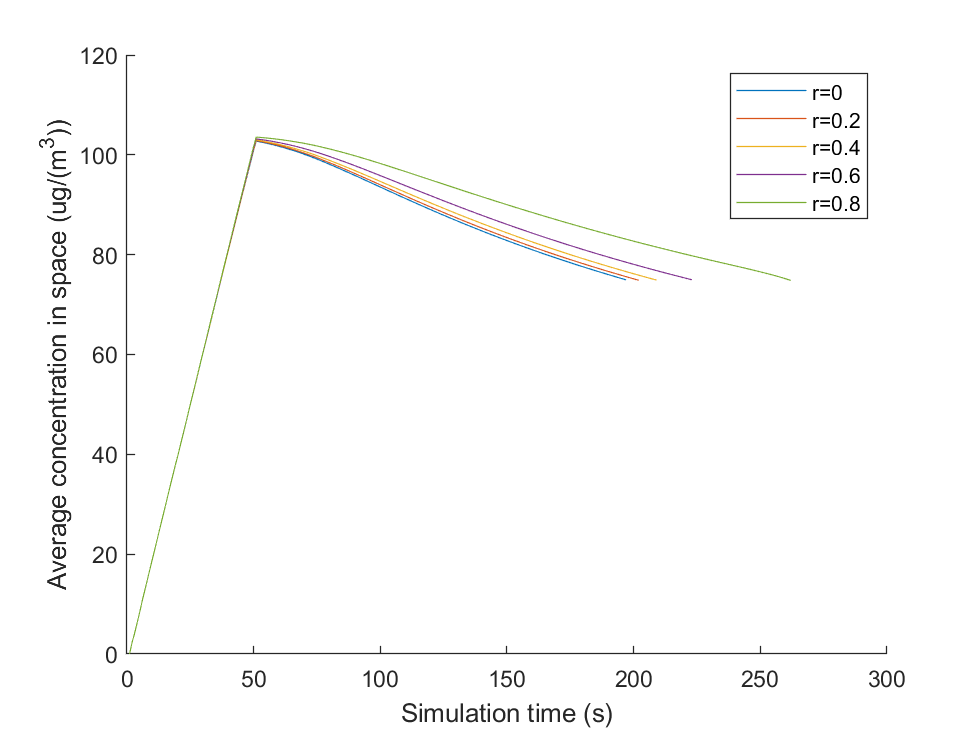
\includegraphics[width=0.6\textwidth]{pics/relation-avg_concentration-t.png}
		\caption{空间平均烟尘浓度-模拟时间关系}
		\label{fig19}
    \end{figure}
    \begin{figure}[htbp]
        \centering
		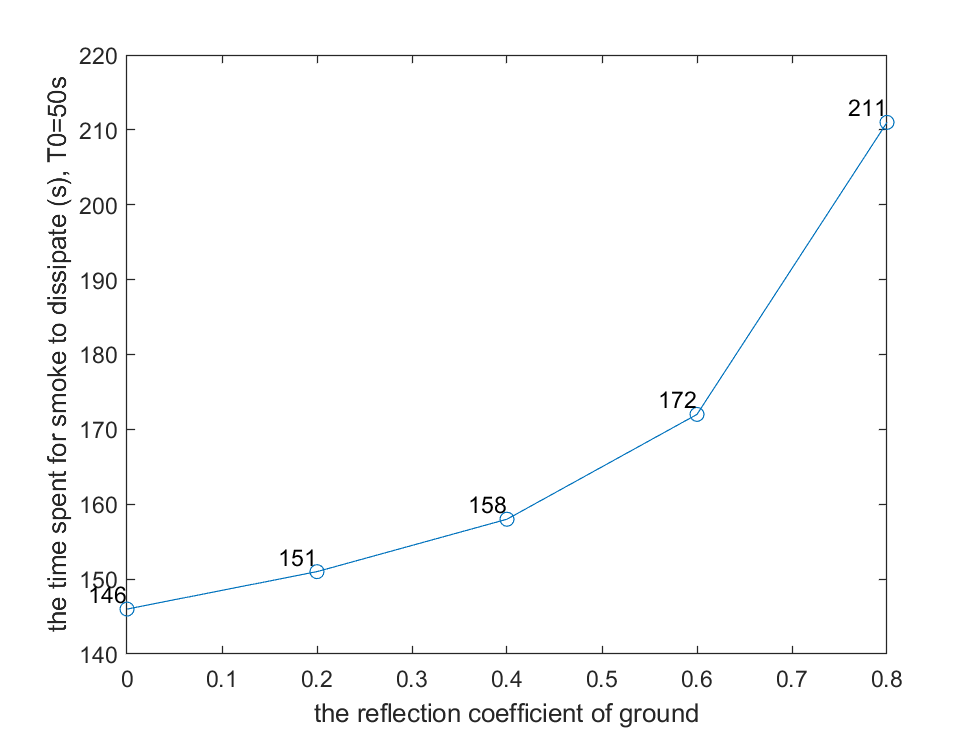
\includegraphics[width=0.6\textwidth]{pics/relation-dissipate_time-r.png}
		\caption{消散时间-地面反射系数关系}
		\label{fig20}
	\end{figure}

	\section{不足与改进}
	\noindent 由于我们模拟烟尘扩散使用有限差分法,并且使用了较多假设,我们可以从中发现如下的不足:
	\begin{itemize}
		\item 几何结构简单:我们假设周围没有其他障碍物,同时高塔本身的体积被忽略.
		\item 气象情况简单:尽管我们已经说明,实际上风速v可以作为有限空间内的一组向量输入,但这会导致计算开销急剧上升.
		\item 模拟精度有限:由于硬件设备的限制,模拟设置的空间大小受到严重的限制.为了提高模拟精度,进一步扩大空间尺度、减小时间步长都将导致设备更大的负载.
		\item 数值模拟局限:尽管很多时候我们仅以极小程度改变某一变量,同时我们可以预测到其对系统的影响较小,但是我们依然需要重新设置参数并从头计算.
		\item 数值问题:实验过程中,我们发现当某些参数,诸如风速$v$和扩散系数$D$超过一定值时,系统将会面临数值问题并崩溃.为了解决这个问题,我们需要减小时间步长$dt$,这将导致不可接受的时间开销;进行浮点数运算时会有数值精度上的误差,偶尔会影响程序中的条件判断.
	\end{itemize}
	为了解决这些问题,我们有如下可能的解决手段,作为未来的工作方向:
	\begin{itemize}
		\item 假设优化:具体考虑到烟尘作为一种混合类型的污染物,应当对将其视为气体扩散这一假设进行检验与修正,同时增加工厂附近的几何和气象信息;另外烟尘在从烟囱出口释放时的更多细节有待加入考量,例如烟尘被释放时应有一定的沿z轴正向的初始动量、烟尘与周围大气之间的温差带来的烟尘抬升效果等等.
		\item 算法改进:在计算资源有限的情况下,优化算法节省开销以达到更高的精度和准确性,同时缩减模拟耗时.
		\item 模型优化:使用经验项,在计算体系过于复杂的情况下,应当使用经验项来代替以简化模型,与实际测量数据进行拟合优化模型.
	\end{itemize}

	\section{组内分工}
	
	\begin{itemize}
		\item 提出假设与建立模型:殷腾
		\item 代码编写与绘图仿真:殷腾、李新涛、郭旭
		\item 结果讨论与报告撰写:殷腾、李新涛、郭旭
	\end{itemize}
	排名顺序不分先后.具体来说,对于本文中\cref{sec6}讨论的多个部分,小组内每人负责一到两部分的全部内容(包括提出、验证、绘图、报告).
	
	\clearpage
	
	\bibliographystyle{ieeetr}
	\begin{thebibliography}{4}
		\item Atkins, Peter, and Loretta Jones. Atkins' Physical Chemistry. 11th edition, OUP Oxford, 2021.\\
		\item 严镇军,数学物理方法.中国科学技术大学出版社,1999.
	\end{thebibliography}
	
	\section*{附录}\addcontentsline{toc}{section}{附录}
	\begin{table}[htbp]
		\centering
		\begin{tabular}{ll}
			diffusion.m & 扩散模拟函数(不包含重力项与地面反射项)\\
			diffusion\_gravity.m & 扩散模拟函数(考虑重力影响)\\
			diffusion\_reflection.m & 扩散模拟函数(考虑地面反射)\\
			visualization.m & 对扩散过程的某次采样进行可视化的函数\\
			& \\
			simulation\_instance & 对一组给定参数的问题实例进行模拟可视化\\
			simulation\_h & 绘制烟囱高度对地面浓度最大值关系图\\
			simulation\_v & 绘制不同风速下地面浓度分布情况图\\
			simulation\_r & 绘制地面反射系数和空气中烟尘消散所需时间关系图\\
			simulation\_w & 绘制重力影响下的地面浓度分布情况\\
		\end{tabular}
		\caption{文件说明}
	\end{table}
	
\end{document}